%----------------------------------------------------------------------------------------
%	PACKAGES AND OTHER DOCUMENT CONFIGURATIONS
%----------------------------------------------------------------------------------------
\documentclass[12pt]{article}
\usepackage{graphicx}
\usepackage{amsmath,amsfonts,stmaryrd,amssymb} % Math packages
\usepackage{bm}
\usepackage{steinmetz}
\usepackage{enumitem}
\graphicspath{{images/}}
\usepackage{float}
\usepackage{hyperref}
\hypersetup{
	colorlinks=true,
	linkcolor=blue,
	filecolor=magenta,      
	urlcolor=cyan,
	pdftitle={Overleaf Example},
	pdfpagemode=FullScreen,
}
\urlstyle{same}
\usepackage{mathtools}
\usepackage{fancyhdr}
\usepackage{xcolor}
\usepackage[american,RPvoltages]{circuiTikz}
\usepackage{tikz, tikz-cd}
\usepackage{pgfplots}
\usepackage{siunitx}
\usetikzlibrary{spy,shapes,arrows, arrows.meta, bending, decorations.markings}
\pgfplotsset{width=10cm,compat=1.18}
\usepackage{lmodern} % package for changing font size
\usepackage{lastpage}
%\renewcommand{\figurename}{Figura}
\usepackage{tcolorbox}
\usepackage{lipsum}
%\usepackage{enumerate} % Custom item numbers for enumerations
\usepackage[ruled]{algorithm2e} % Algorithms
\usepackage[framemethod=tikz]{mdframed} % Allows defining custom boxed/framed environments
\usepackage{listings} % File listings, with syntax highlighting
%\lstset{basicstyle=\ttfamily,} % Typeset listings in monospace font
\usepackage{lipsum}
\tcbuselibrary{listings,theorems,skins,vignette,raster,breakable,magazine,poster,fitting,hooks}
\usepackage[T1]{fontenc}
\usepackage{tgbonum}
 \fontfamily{garamond}
\definecolor{myblue}{RGB}{24, 51, 73}
%----------------------------------------------------------------------------------------
%	DOCUMENT MARGINS
%----------------------------------------------------------------------------------------

\usepackage{geometry} % Required for adjusting page dimensions and margins
\geometry{
	paper=a4paper, % Paper size, change to letterpaper for US letter size
	top=2.5cm, % Top margin
	bottom=3cm, % Bottom margin
	left=2cm, % Left margin
	right=2.5cm, % Right margin
	headheight=14pt, % Header height
	footskip=1.5cm, % Space from the bottom margin to the baseline of the footer
	headsep=1.2cm, % Space from the top margin to the baseline of the header
	%showframe, % Uncomment to show how the type block is set on the page
}

%----------------------------------------------------------------------------------------
%	FONTS
%----------------------------------------------------------------------------------------

\usepackage[utf8]{inputenc} % Required for inputting international characters
\usepackage[T1]{fontenc} % Output font encoding for international characters
\usepackage{XCharter} % Use the XCharter fonts
\usepackage{tgbonum}

\makeatletter
\pgfcircdeclarebipole{}{\ctikzvalof{bipoles/vsourcesin/height}}{sVpm}{\ctikzvalof{bipoles/vsourcesin/height}}{\ctikzvalof{bipoles/vsourcesin/width}}{
	
	\pgfsetlinewidth{\pgfkeysvalueof{/tikz/circuitikz/bipoles/thickness}\pgfstartlinewidth}
	\pgfpathellipse{\pgfpointorigin}{\pgfpoint{0}{\pgf@circ@res@up}}{\pgfpoint{\pgf@circ@res@left}{0}}
	\pgfusepath{draw}     
	\pgftext[bottom,rotate=90,y=\ctikzvalof{bipoles/vsourceam/margin}\pgf@circ@res@down]{\scriptsize$-$}
	\pgftext[top,rotate=90,y=\ctikzvalof{bipoles/vsourceam/margin}\pgf@circ@res@up]{\scriptsize$+$}
	
	\pgf@circ@res@up = .35\pgf@circ@res@up
	\pgfscope
	\pgftransformrotate{90}
	\pgfpathmoveto{\pgfpoint{-\pgf@circ@res@up}{0cm}}
	\pgfpathsine{\pgfpoint{.5\pgf@circ@res@up}{.4\pgf@circ@res@up}}
	\pgfpathcosine{\pgfpoint{.5\pgf@circ@res@up}{-.4\pgf@circ@res@up}}
	\pgfpathsine{\pgfpoint{.5\pgf@circ@res@up}{-.4\pgf@circ@res@up}}
	\pgfpathcosine{\pgfpoint{.5\pgf@circ@res@up}{.4\pgf@circ@res@up}}
	\pgfusepath{draw}
	\endpgfscope
}
\def\pgf@circ@sVpm@path#1{\pgf@circ@bipole@path{sVpm}{#1}}
\compattikzset{sinusoidal voltage source pm/.style = {\circuitikzbasekey, /tikz/to path=\pgf@circ@sVpm@path, \circuitikzbasekey/bipole/is voltage=true, \circuitikzbasekey/bipole/is voltageoutsideofsymbol=true, v=#1 }}
\compattikzset{sVpm/.style = {\comnpatname sinusoidal voltage source pm = #1}}

\pgfcircdeclarebipole{}{\ctikzvalof{bipoles/vsourcesin/height}}{sVpmh}{\ctikzvalof{bipoles/vsourcesin/height}}{\ctikzvalof{bipoles/vsourcesin/width}}{
	
	\pgfsetlinewidth{\pgfkeysvalueof{/tikz/circuitikz/bipoles/thickness}\pgfstartlinewidth}
	\pgfpathellipse{\pgfpointorigin}{\pgfpoint{0}{\pgf@circ@res@up}}{\pgfpoint{\pgf@circ@res@left}{0}}
	\pgfusepath{draw}     
	\pgftext[center,x=0.2\pgf@circ@res@down-\ctikzvalof{bipoles/vsourceam/margin}\pgf@circ@res@down]{\scriptsize$-$}
	\pgftext[top,rotate=90,y=\ctikzvalof{bipoles/vsourceam/margin}\pgf@circ@res@up]{\scriptsize$+$}
	
	\pgf@circ@res@up = .35\pgf@circ@res@up
	\pgfscope
	\pgftransformrotate{90}
	\pgfpathmoveto{\pgfpoint{-\pgf@circ@res@up}{0cm}}
	\pgfpathsine{\pgfpoint{.5\pgf@circ@res@up}{.4\pgf@circ@res@up}}
	\pgfpathcosine{\pgfpoint{.5\pgf@circ@res@up}{-.4\pgf@circ@res@up}}
	\pgfpathsine{\pgfpoint{.5\pgf@circ@res@up}{-.4\pgf@circ@res@up}}
	\pgfpathcosine{\pgfpoint{.5\pgf@circ@res@up}{.4\pgf@circ@res@up}}
	\pgfusepath{draw}
	\endpgfscope
}
\def\pgf@circ@sVpmh@path#1{\pgf@circ@bipole@path{sVpmh}{#1}}
\compattikzset{sinusoidal voltage source pmh/.style = {\circuitikzbasekey, /tikz/to path=\pgf@circ@sVpmh@path, \circuitikzbasekey/bipole/is voltage=true, \circuitikzbasekey/bipole/is voltageoutsideofsymbol=true, v=#1 }}
\compattikzset{sVpmh/.style = {\comnpatname sinusoidal voltage source pmh = #1}}
\makeatother


%----------------------------------------------------------------------------------------
%	BEGIN DOCUMENT
%----------------------------------------------------------------------------------------

\begin{document}
	%\thispagestyle{empty}
	\begin{tikzpicture}[remember picture, overlay]
		\node[anchor=north west, inner sep=0pt] at (current page.north west) {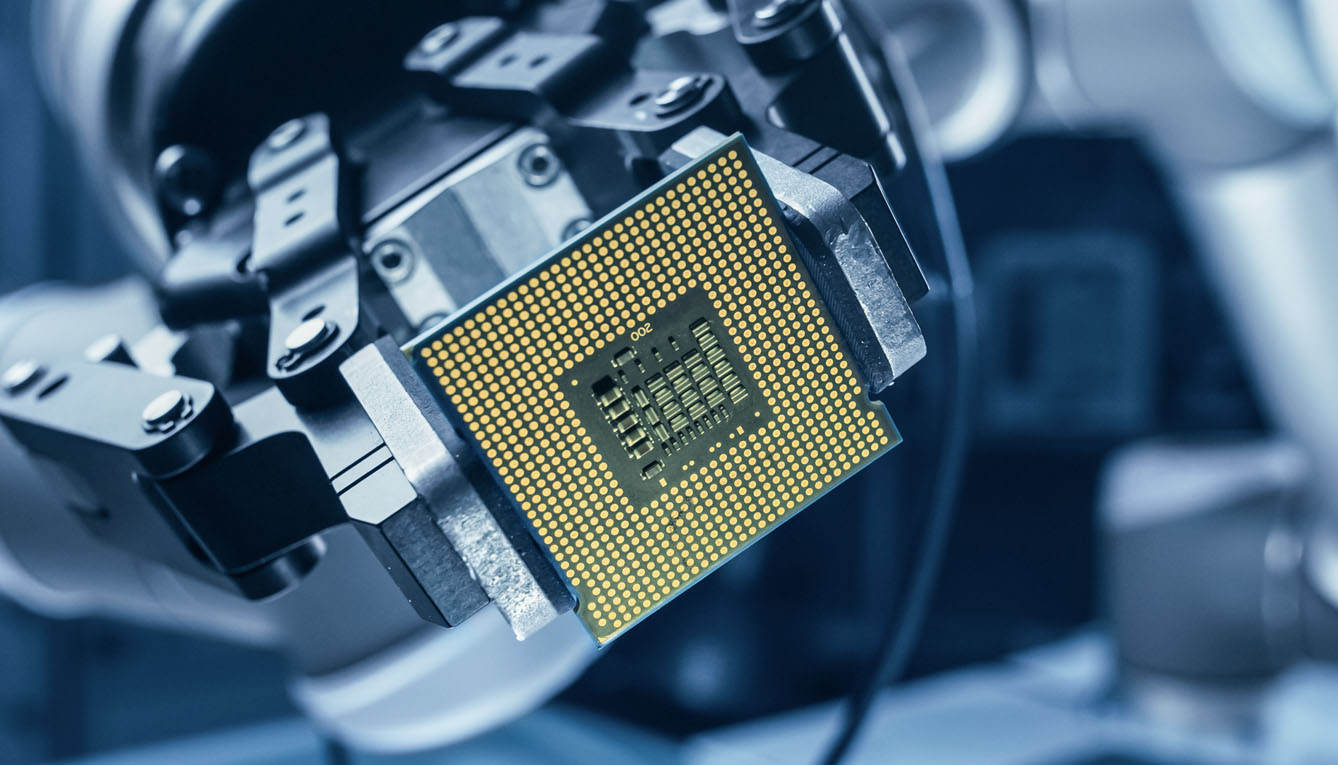
\includegraphics[width=\paperwidth, height=.5\paperheight]{picture1}};
	\end{tikzpicture}

	\vspace{13cm}
	\noindent \textcolor{myblue}{\fontsize{40pt}{40pt}\selectfont \textbf{Análisis de amplificador cascode con BJTs}}\\\\\\
	{\fontsize{18pt}{18pt}\selectfont Agosto, 2023} 
	
	\newpage
	\begin{figure}[H]
		\centering	
		\begin{tikzpicture}[scale=0.8]

			\draw (0,0) node[npn,right](Q1){$Q_1$};
			\draw (Q1.B) to[R, l_=$R_B$, i_<=$I_B$] ++(-5,0) to [V, invert, l_=$V_{BB}$] ++(0,-4) node[ground]{};
			\draw (Q1.E) to[short] ++(0,-2) node[ground]{};
			\draw (Q1.C) to[short, -*, i<=$I_C$] ++(0,1) coordinate(c1) to[L, i^<=$I_1$, l=$L_1$] ++(0,4);
			\draw (c1) to[short] ++(-2,0) to[full diode, l=$D_1$] ++(0,4) to[short, -*] ++(2,0) coordinate (c2);
			\draw (c1) to[short] ++(2,0);
			\draw (c2) to[short, i=$I_{LED}$] ++(2,0) to[R, l=$R_{LED}$] ++(0,-2) to[led, fill=red, l=$LED_1$] ++(0,-2);
			\draw (c2) to[short] ++(0,0.5) node[vcc]{$V_{CC}$};
			\draw (-0.5,0) node[below]{$+$};
			\draw (0.6,-1) node[below]{$-$};
			\draw (0.1,-0.4) node[below]{$V_{BE}$};
			%\draw (Q1.C) to[R, l=$R_C$, i<=$I_C$] ++(0,5) node[vcc]{$V_{CC}$};
		\end{tikzpicture}
		\caption{Transistor Switch}	
		\label{fig:figura1}
	\end{figure}


\begin{align}
	V_{BB} - R_BI_B - V_{BE} = 0 \nonumber \\
	R_B = \frac{ V_{BB} - V_{BE_{(sat)}} }{ I_B }
\end{align}
 
Where

\begin{align}
	I_B = \frac{I_C}{\beta_{forced}}
\end{align}

\noindent Assuming $B_{forced} = 20$, $V_{BB}$ = \qty{3.3}{\volt}, $V_{CC}$ = \qty{5}{\volt}, $V_{BE_{(sat)}}$ = \qty{0.7}{\volt}, $I_{LED}$ = \qty{20}{\milli \ampere} and $I_1$ =  \qty{170}{\milli \ampere} then:
\begin{align}
	I_B = \frac{I_C}{\beta_{forced}} = \frac{\qty{190}{\milli \ampere}}{20} = \qty{9.5}{\milli \ampere}
\end{align}

Where
\begin{align}
	I_C= I_1 + I_{LED}
\end{align}

Then

\begin{align}
	R_B = \frac{\qty{3.3}{\volt} - \qty{0.7}{\volt}}{\qty{9.5}{\milli \ampere}} = \qty{273.7}{\ohm} \approx \qty{270}{\ohm}
\end{align}

Finally
\begin{align}
	R_{LED} = \frac{V_{CC} - V_{LED} - V_{CE_{(sat)}}}{I_{LED}} = \frac{ \qty{5}{\volt} - \qty{2}{\volt} - \qty{0.2}{\volt} }{ \qty{20}{\milli \ampere} } = \qty{140}{\ohm}
\end{align}
\end{document}
